The persistence API provides abstracted access to a persistence provider while
remaing decoupled from the underlying technology, including but not limited to
database, SQL version and transaction management, whilst employing a range of
software engineering tactics to concretely address required quality
requirements required for the persistence domain.

\subsection{Architecture Requirements}
The architectural requirements for the persistence API include the refined
quality requirements and architectural requirements listed below. The
architectural constraints for this lower level components are the same as for
the system as whole, as referred to in
section \ref{sec:systemArchitecturalConstraints} with further extensions as
specified in section \ref{sec:persistenceAPIArchitecturalConstraints}.

\subsubsection{Quality Requirements}
\paragraph{Flexibility}
The provided persistence API should be able to adapt to the rapidly evolving
persistence architecture domain, especially in terms of the different
methodologies of storing data such as relational and NoSQL data stores. It is
further import that the persistence layer is not locked to any specific
persistence technology.

Further the chosen API should to force the use of any vendor specific
transaction management, but should rather provide an abstraction layer allowing
the use of any transaction manager implementing the required interface.

\paragraph{Maintainability}
\label{sec:persistenceAPIMaintainability}
The used persistence API should be in a mature stage of the software development
life cycle as to guard against a rapidly evolving changing API. The chosen
persistence API should be an open standard with multiple realization as to guard
against realization technologies be abandoned. This will allow in future an easier
switch to another persistence API implementation if required for the long term
maintance and use of the project.

\paragraph{Scalability}
The chosen persistence API should be able to allow for future scaling of the
infrastructure either horizontally or vertically with a preference for
horizontal scaling.

\paragraph{Performance}
The persistence API should allow for the use of certain architectural tactics
to increase performance. Specifically the following tactics should be supported
to some extent
\begin{itemize}
	\item Object Caching
	\item Connection Pooling
	\item Thread Provisioning
	\item Scheduling
\end{itemize}

\paragraph{Reliability}
The chosen API should allow security at least providing authorization on
entities managed by the underlying persistence technology architecture.

\subsubsection{Architectural Responsibilities}
The architectural responsibilities of the persistence API are shown in
Figure \ref{fig:persistenceResponsibilities}
\begin{figure}[H]
	\begin{center}
	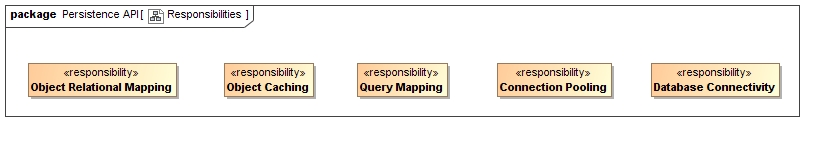
\includegraphics[scale=0.5]{../Diagrams and Charts/Persistence API/Responsibilities.jpg}
	\caption{The architectural responsibilities of the Persistence API}
	\label{fig:persistenceResponsibilities}
	\end{center}
\end{figure}

\subsubsection{Architecture Constraints}
The chosen persistence API should be a currently active standard, with a medium
to large sized active community supporting the standard and should be realized
by at least three active realizations of the chosen API as to ensure future
maintainability as set out by the required quality requirement in
section \ref{sec:persistenceAPIMaintainability}.
\label{sec:persistenceAPIArchitecturalConstraints}

\subsection{Architecture Design}
\subsubsection{Tactics}
The persistence API implement the following tactics:
\begin{itemize}
	\item \textit{Object Relational Mapping} to reduce code bulk, improve
		maintainability and allow for decoupling from the persistence
		provider.
	\item \textit{Query Mapping} from queries across a graph of Java objects
		onto the database queries used in the selected database
		technology and provider.
	\item \textit{Object caching} to improve scalability and performance.
	\item \textit{Transactions} with 2-phase commit to improve reliability
		of processes.
	\item \textit{Transaction Neutral API} allow the use of any transaction manager
		implementing the required interface as to improve flexibility and
		future maintainability.
	\item \textit{Connection Pooling} to improve performance and scalability.
\end{itemize}

\subsubsection{Architectural Components}
The architectural components of the persistence API are shown in Figure \ref{fig:persistenceResponsibilityAllocation}
\begin{figure}[H]
	\begin{center}
	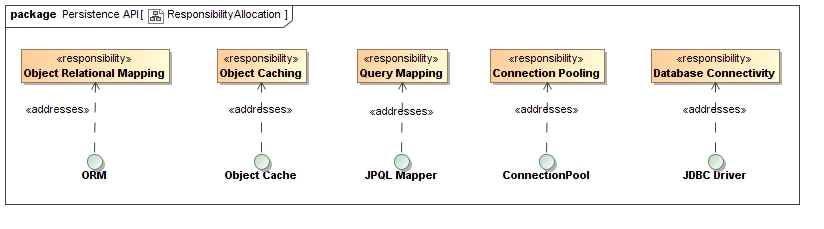
\includegraphics[scale=0.5]{../Diagrams and Charts/Persistence API/ResponsibilityAllocation.jpg}
	\caption{The abstract components to which the architectural responsibilities are assigned.}
	\label{fig:persistenceResponsibilityAllocation}
	\end{center}
\end{figure}

\subsubsection{Frameworks and Technologies}
A JPA 2.1 (Java Persistence API Version 2.1) provider will be used as a
persistence API. The chosen concrete implementation used will be Hibernate as
it has support for both relational and NoSQL persistence providers.

The JPA 2.1 API is a widely supported public standard which are implemented by
the following products:
\begin{itemize}
	\item Hibernate
	\item EclipseLink
	\item DataNucleus
\end{itemize}

Further more the listed implementations all support the use of NoSQL databases
by utilizing the JPA standard for relational databases. Thus the required
quality requirements of using an open standard with multiple implementations
supporting both relational and NoSQL database are fulfilled.

The persistence context (EntityManager) will will be dependency injected into
services requiring access to persistent data. JPA providers do implement
\begin{itemize}
	\item \textit{Object Relational Mapping} including the mapping of
		relationships between objects via a provided ORM
		implementation such as Hibernate or EclipseLink.
	\item \textit{Query Mapping} from object-oriented queries across the
		domain object graph to queries for a specific database provider.
	\item \textit{Object caching} within the persistence context with
		in-memory or NoSQL database based caching allow for the
		fulfilment of the performance, flexibility and scalability
		quality requirements.
	\item \textit{Transactions} are supported through the use of the \textit{Java Transaction API (JTA)}.
	\item \textit{Transaction Neutral API} is supported through the Spring
		Framework transaction manager supporting a consistent programming
		model across different transaction APIs such as
		Java Transaction API, JDBC, Hibernate, Java Persistence API and
		Java Data Objects.
	\item \textit{Connection Pooling} is provided through a JCA connector
		based implementation of a JDBC driver.
\end{itemize}

Queries will be specified as Spring Data JPA queries, thereby reducing
boilerplate code which ease future maintenance and development, as the queries
are not specific to any underlying query language e.g. SQL or any underlying
persistence technology such as relational or NoSQL providers.

\paragraph{Concepts and Constraints for Application Components}
The application concepts within the persistence domain include
\begin{itemize}
	\item \textit{Domain objects} which host long-living state objects, and is realized in the Java architecture as Plain Old Java Objects (POJO's) which doesn't contain any business logic.
	\item \textit{Queries across object graph of domain objects} through which the required information of state in the domain objects is retrieved, modified and removed.
\end{itemize}